\documentclass[a4paper,11pt,russian]{extreport}
% Эта строка — комментарий, она не будет показана в выходном файле
\usepackage[T2A]{fontenc}
\usepackage[utf8]{inputenc} % Включаем поддержку UTF8
\usepackage[russian]{babel}%используем русский и английский языки с переносами
\usepackage{enumerate}
\usepackage{etoolbox}
\usepackage{amsmath}
\usepackage{listings}
\usepackage{pgfplots}
\usepackage{pgfplotstable}
\pgfplotsset{every axis legend/.append style={
		at={(1,1)},
		anchor=north west}}


\usepackage{titlesec}
\titleformat{\chapter}[block]
{\Huge\bfseries}{\thechapter}{10pt}{\Huge}

\usepackage[left=3cm,right=3cm,
top=2cm,bottom=2cm]{geometry}

\lstset{numbers=left}

\newcommand*{\No}{\textnumero}

\begin{document}
	\begin{titlepage}
		\begin{center} 
			Государственное образовательное учреждение высшего профессионального образования
			
			
			«Московский Государственный Технический Университет имени Н. Э. Баумана»
		\end{center}
		\vspace*\fill
		\begin{center}
			\scshape\LARGE {
				Отчет по лабораторной работе \No 2\\
				<<Интервальные оценки>> \\
				по курсу <<Математическая статистика>>\\
				}
			\scshape\Large{Вариант 1 \\}
			\vspace{1cm}
			\scshape\Large{
				Студент: Анисимов Н.С. ИУ7-62 \\
				Преподаватель: Велищанский М.А.\\ }
			
		\end{center}
		\vspace*\fill
		\centering\today
	\end{titlepage}
	
	\tableofcontents
	
	\newpage
	
	\chapter{Формулы и определения}
	
	
	\section{Доверительный интервал}
	Доверительным интервалом уровня \(\gamma\) ( \(\gamma\)-доверительным интервалом) для параметра \(\Theta\) называют пару статистик \(\underline{\Theta}(\vec{X_n})\), \(\overline{\Theta}(\vec{X_n})\) таких, что \(P\{\Theta \in [\underline{\Theta}(\vec{X_n}), \overline{\Theta}(\vec{X_n})] \} = \gamma \) . Другими словами, \(\gamma\)-доверительный интервал – интервал, который покрывает теоретическое значение параметра \(\Theta\) с вероятностью \(\gamma\).
	
	Односторонней нижней--доверительной границей для параметра \(\Theta\) называется статистика \(\underline{\Theta}(\vec{X_n})\) такая, что \(P\{\Theta \in [\underline{\Theta}(\vec{X_n}),+\infty) \} = \gamma \).
	
	Односторонней верхней--доверительной границей для параметра \(\Theta\) называется статистика \(\underline{\Theta}(\vec{X_n})\) такая, что \(P\{\Theta \in (-\infty, \overline{\Theta}(\vec{X_n})] \} = \gamma \).
	
	
	\section{\boldmath Формулы для вычисления границ $\gamma$-доверительного интервала}
	
	
	\paragraph{Оценка для математического ожидания при известной дисперсии} 	\mbox{}\\
	\(\mu \) - неизвестна, \(\sigma^2\) - известна
	
	\begin{align}
	\underline{\mu}(\vec{X}_{n}) &= \overline{X}-\frac{\sigma u_{1-\alpha}}{\sqrt{n}},\\
	\overline{\mu}(\vec{X}_{n}) &= \overline{X}+\frac{\sigma u_{1-\alpha}}{\sqrt{n}}
	\end{align}
	
	\paragraph{Оценка для математического ожидания при неизвестной дисперсии}	\mbox{}\\
	\(\mu \) - неизвестна, \(\sigma^2\) - неизвестна
	
	\begin{align}
	\underline{\mu}(\vec{X}_{n}) &= \overline{X}-\frac{S(\vec{X}_{n})t_{1-\alpha}}{\sqrt{n}},\\
	\overline{\mu}(\vec{X}_{n}) &= \overline{X}+\frac{S(\vec{X}_{n})t_{1-\alpha}}{\sqrt{n}}
	\end{align}
	
	\paragraph{Оценка для дисперсии}	\mbox{}\\
	\(\mu \) - неизвестна, \(\sigma^2\) - неизвестна
	
	\begin{align}
	\underline{\sigma^{2}}(\vec{X}_{n}) & =\frac{S(\vec{X}_{n})(n-1)}{h_{1-\alpha}},\\
	\overline{\sigma^{2}}(\vec{X}_{n}) & =\frac{S(\vec{X}_{n})(n-1)}{h_{\alpha}}
	\end{align}
	
	\noindent где:
	\begin{itemize}
		\item $\alpha = \frac{1-\gamma}{2}; u_a, t_a, h_a$ -- квантили уровня \(\alpha\) нормального распределения, распределения Стьюдента и распределения \(\chi\)-квадрат соответственно; $n$ -- объем выборки.
	\end{itemize}
	
	
	
	\chapter{Листинг}
	\lstinputlisting[language=MatLab]{../src/l2.m}
	
	\chapter{\boldmath Результаты ($\gamma = 0.9$)}
	\begin{align*}
	\mu =& -1.76 \\
	S^2 =& = 1.03 \\ \\
	\mu_{low} =& -1.76 \\
	\mu_{high} =& -1.45 \\
	\hat{\sigma}^2_{low} =&  0.85 \\
	\hat{\sigma}^2_{high} =& 1.30 \\
	\end{align*}
	
	\begin{figure}
		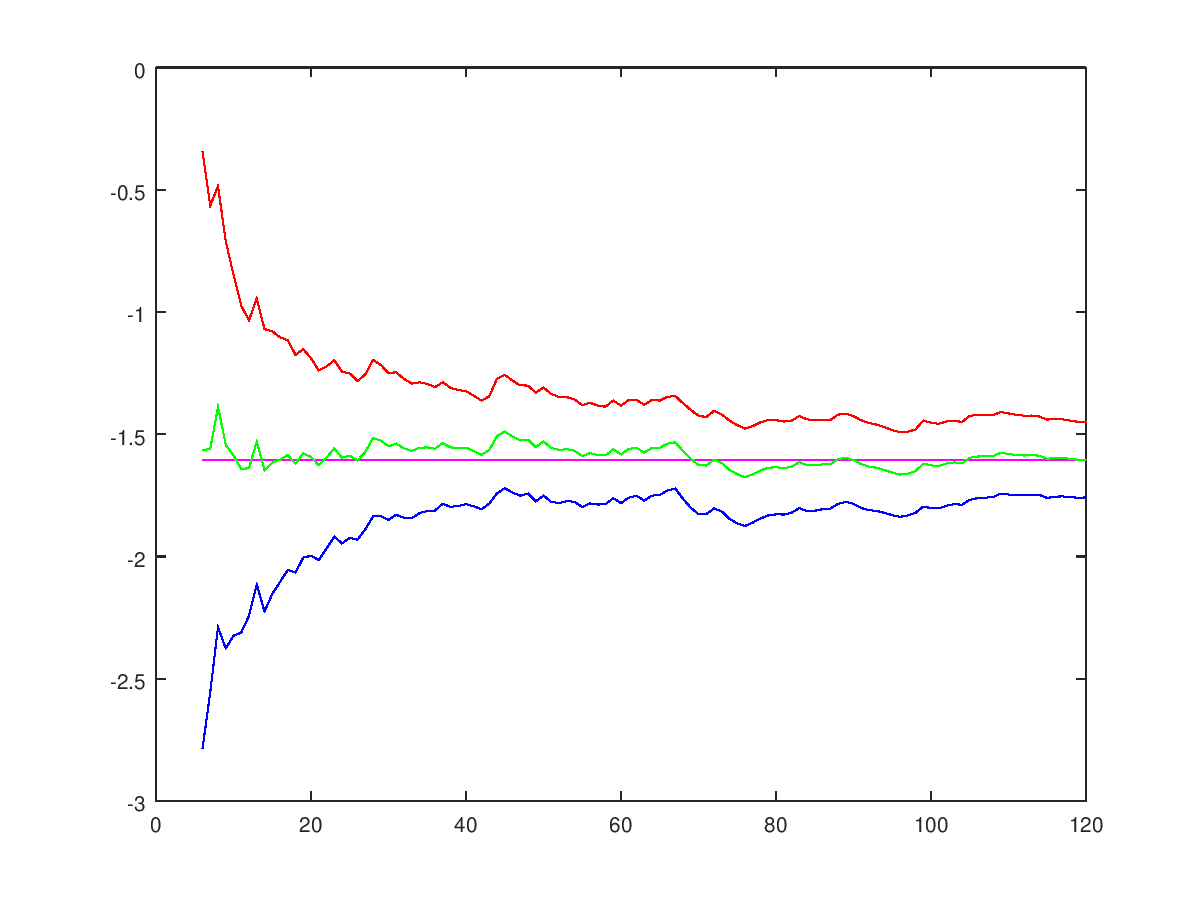
\includegraphics[width=\linewidth]{../img/3.png}
		\caption{Графики математического ожидания}
		\label{fig:1}
	\end{figure}
	
	\begin{figure}
		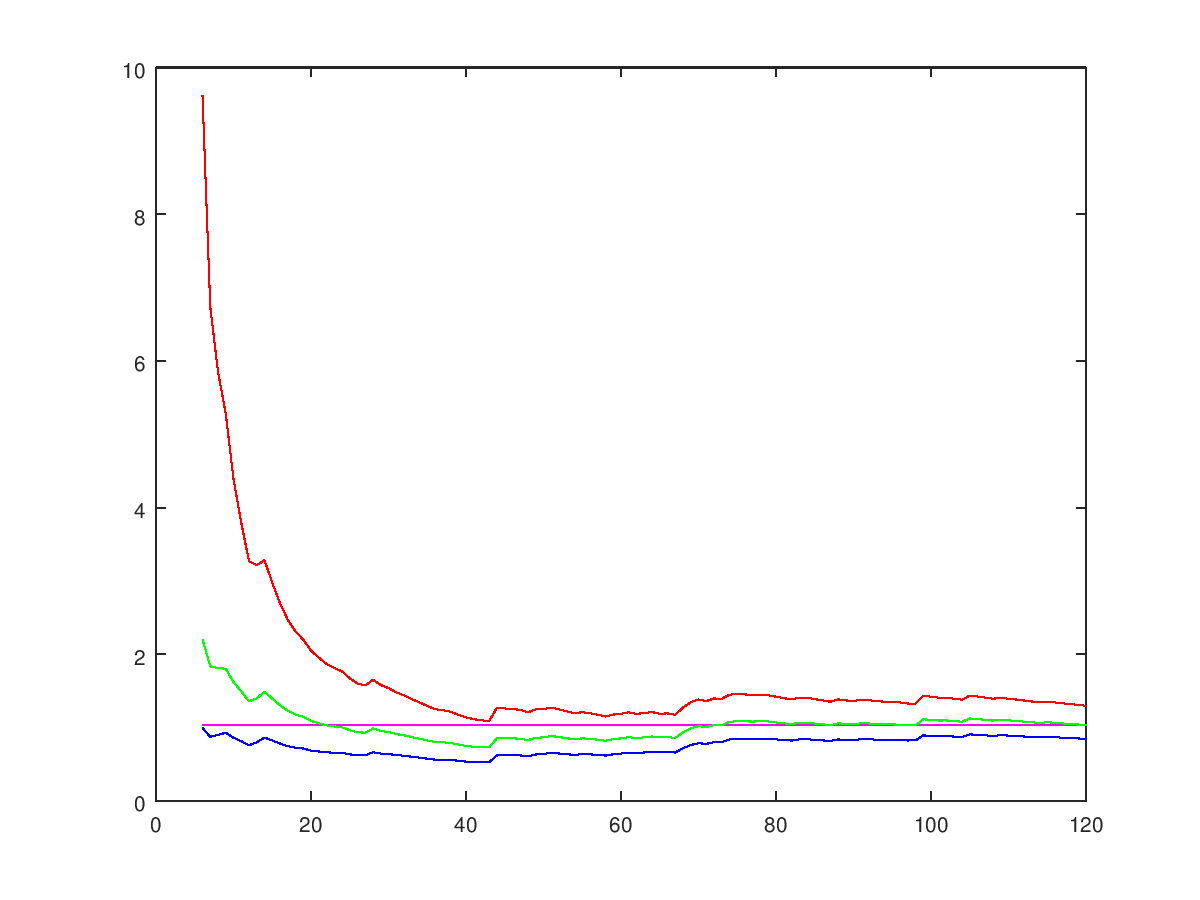
\includegraphics[width=\linewidth]{../img/2.png}
		\caption{Графики дисперсии}
		\label{fig:2}
	\end{figure}
	
		
	
\end{document}